\section{算法介绍} \label{algo}
\subsection{基于网络流的布线方案}
\qquad
首先分析可以知道,题目可以抽象为给定一张图,寻找一些点不相交路径,使得总长度最短。

现在对于棋盘中的每个节点$u$,由于只能经过一次,将其拆成两个节点$u_{in}, u_{out}$,分别表示进入这个节点的边和从这个节点出去的边。连接一条费用为$0$,流量为$1$的边$(u_{in}, u_{out})$来表示节点只能经过一次的这个限制。

另外对于每一个节点,由于可以向其相邻节点前进,因此对于每一对相邻的节点$(u, v)$,连接一条费用为$1$,流量为$1$的从$(u_{out}, v_{in})$的边。

此外对于每一个内部节点$u$,从源$s$向$u_{in}$连接一条费用为$0$,流量为$1$的边,对于每一个边界节点$v$,从$v_{out}$向汇$t$连接一条费用为$0$,流量为$1$的边。

这样,计算最小费用最大流之后就可以得到最优方案了。

此外还有一个关于最小电路板大小的问题,可以利用二分答案来进行计算。即每次判断这个网络是否满流,而这个计算过程中只需要判断合法性而无需最优性,我们可以利用最大流算法而忽略费用以提高速度。
\subsection{基于规则的布线方案}
\qquad
该方法的所有源代码均在route\_rule\_based.h和route\_rule\_based.cpp中。整体的思路是将整个正方形区域划分成四个小块分别对其进行处理,最后将其合并成一整张图。就像这样:

\begin{figure}[H]
	\centering
	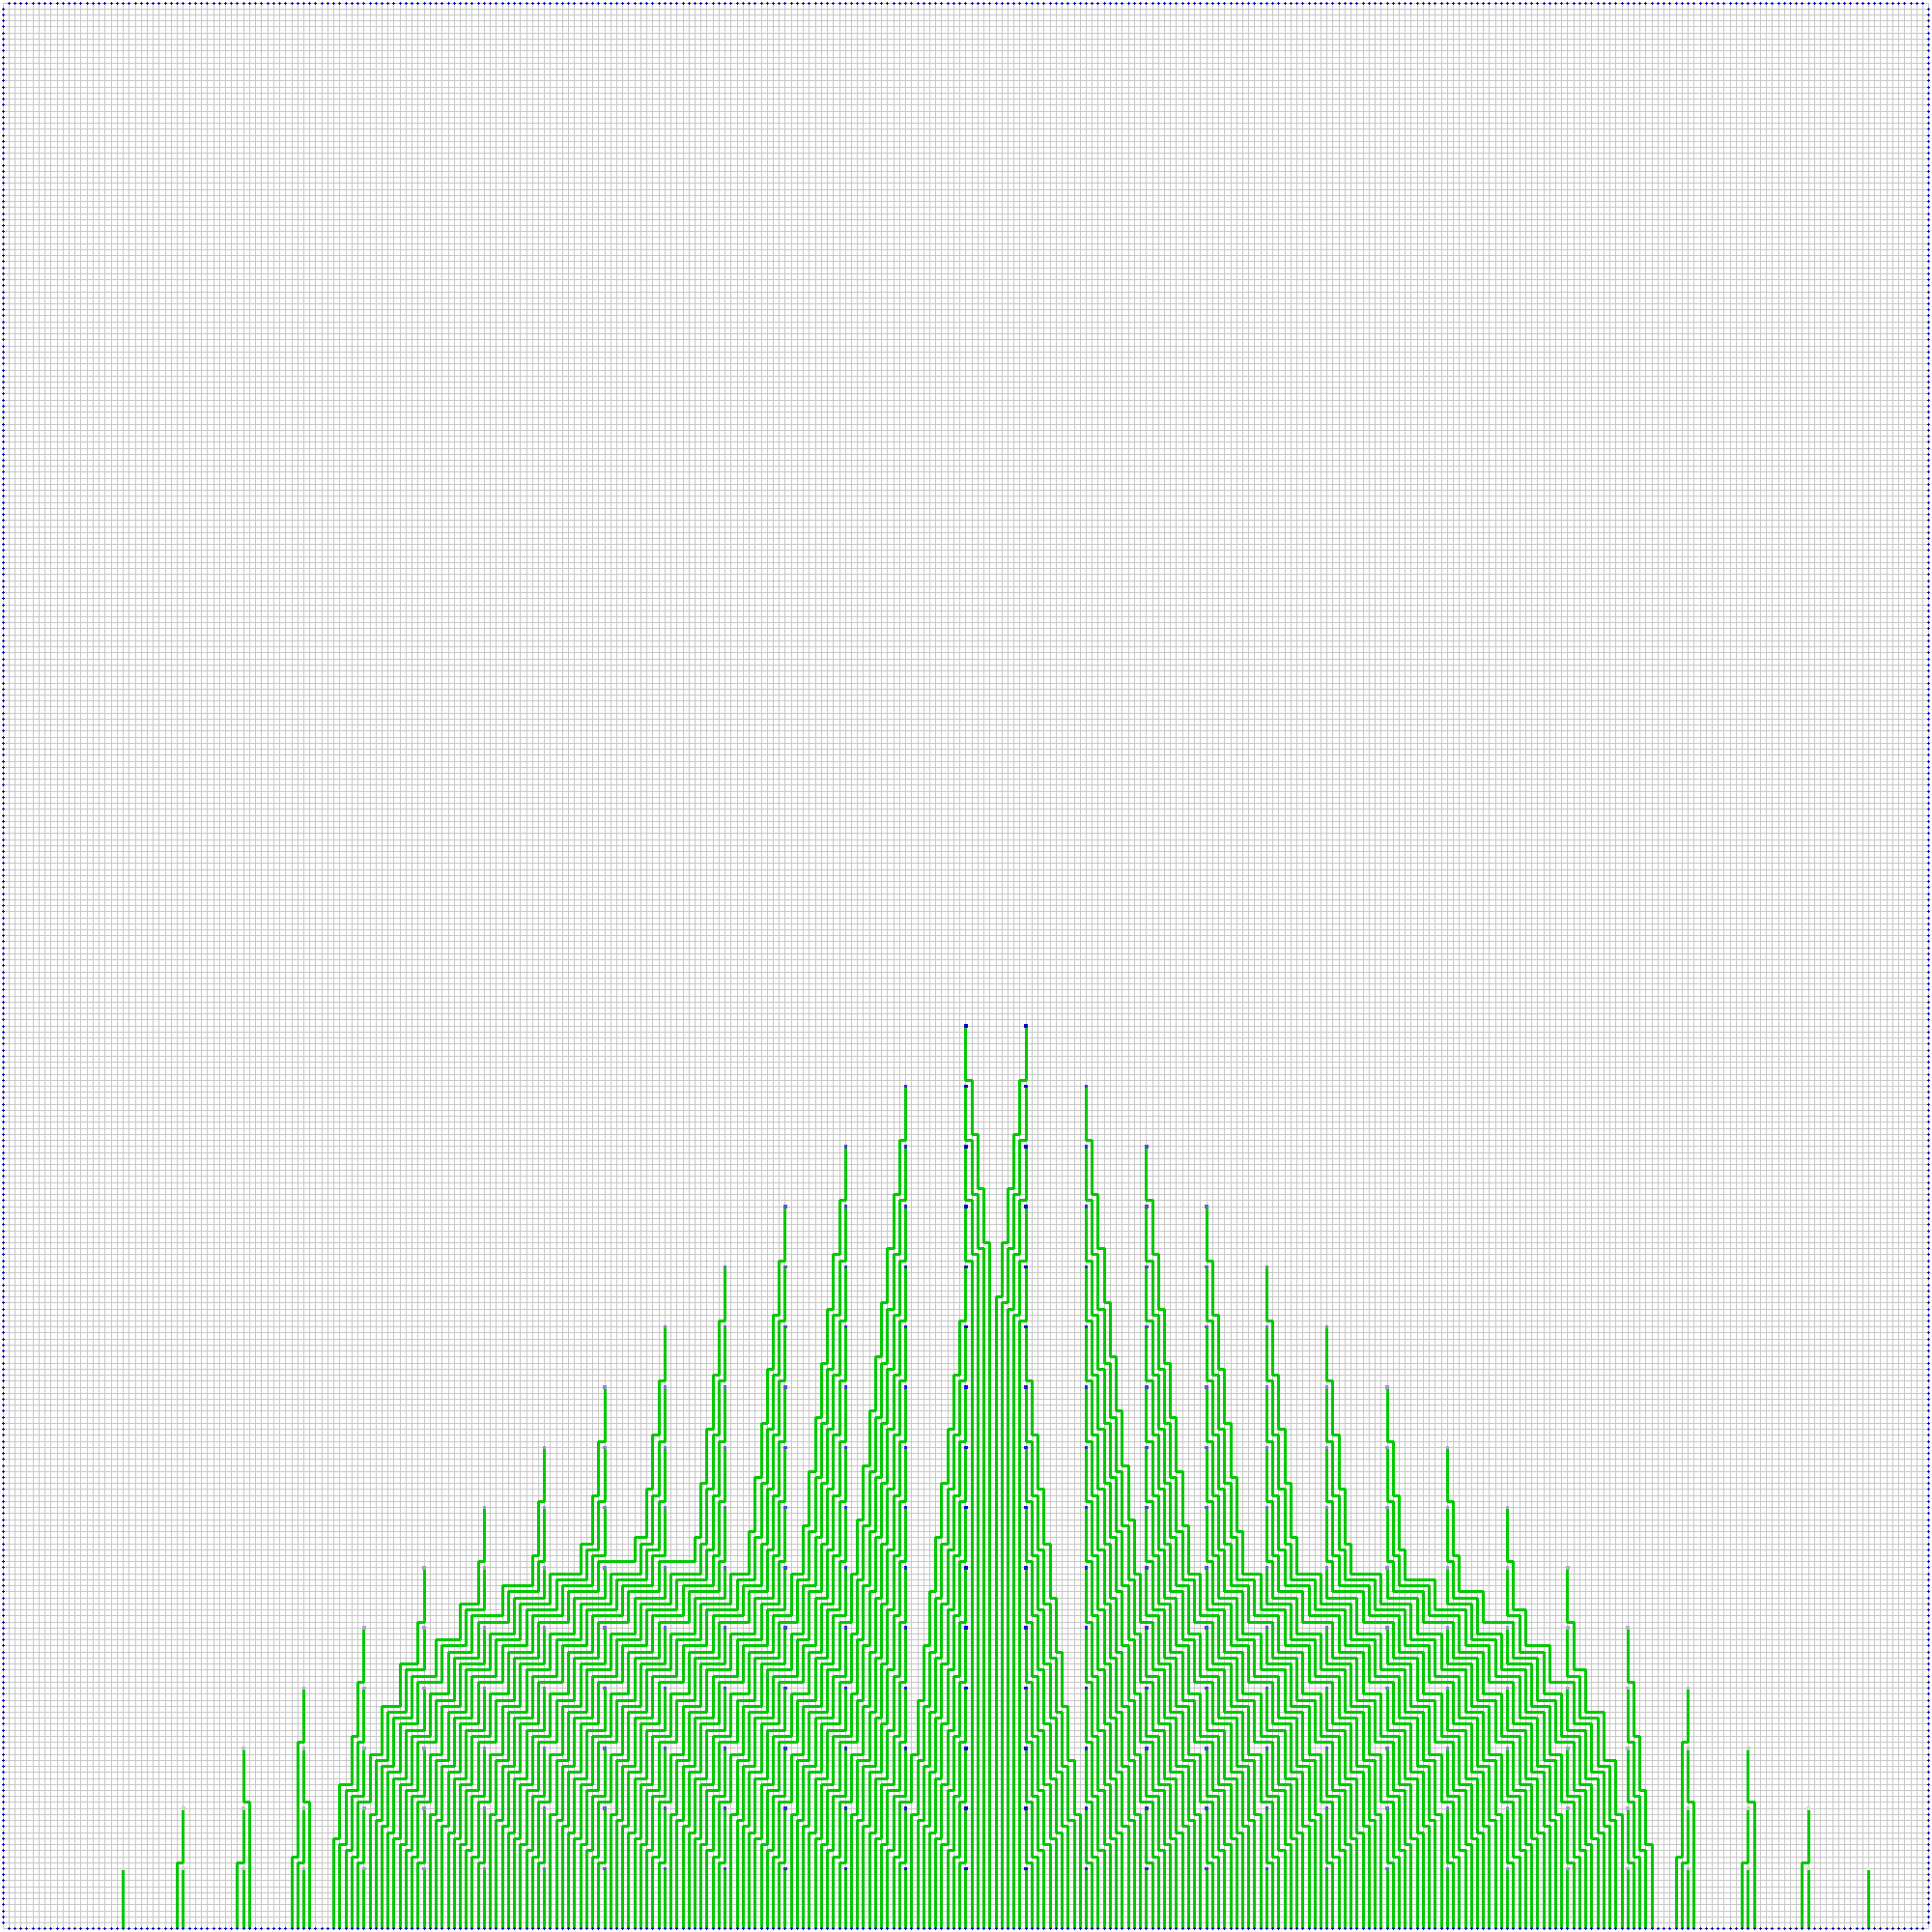
\includegraphics[width=2in]{31.png}
\end{figure}

下半部的三角形会如法炮制地在左部、右部和上部生成,从而构成结果。

\subsubsection{算法设计}
\qquad
\begin{enumerate}
	\item 将正方形点集划分为四个三角形区域,尽量保证均匀划分。以下只考虑在一个三角形内部的情况。
	\item 将最外侧的点直接连出去。由于间隔数的限制,可以证明这些点在最优解下一定只有如下方案。
	\begin{figure}[H]
		\centering
		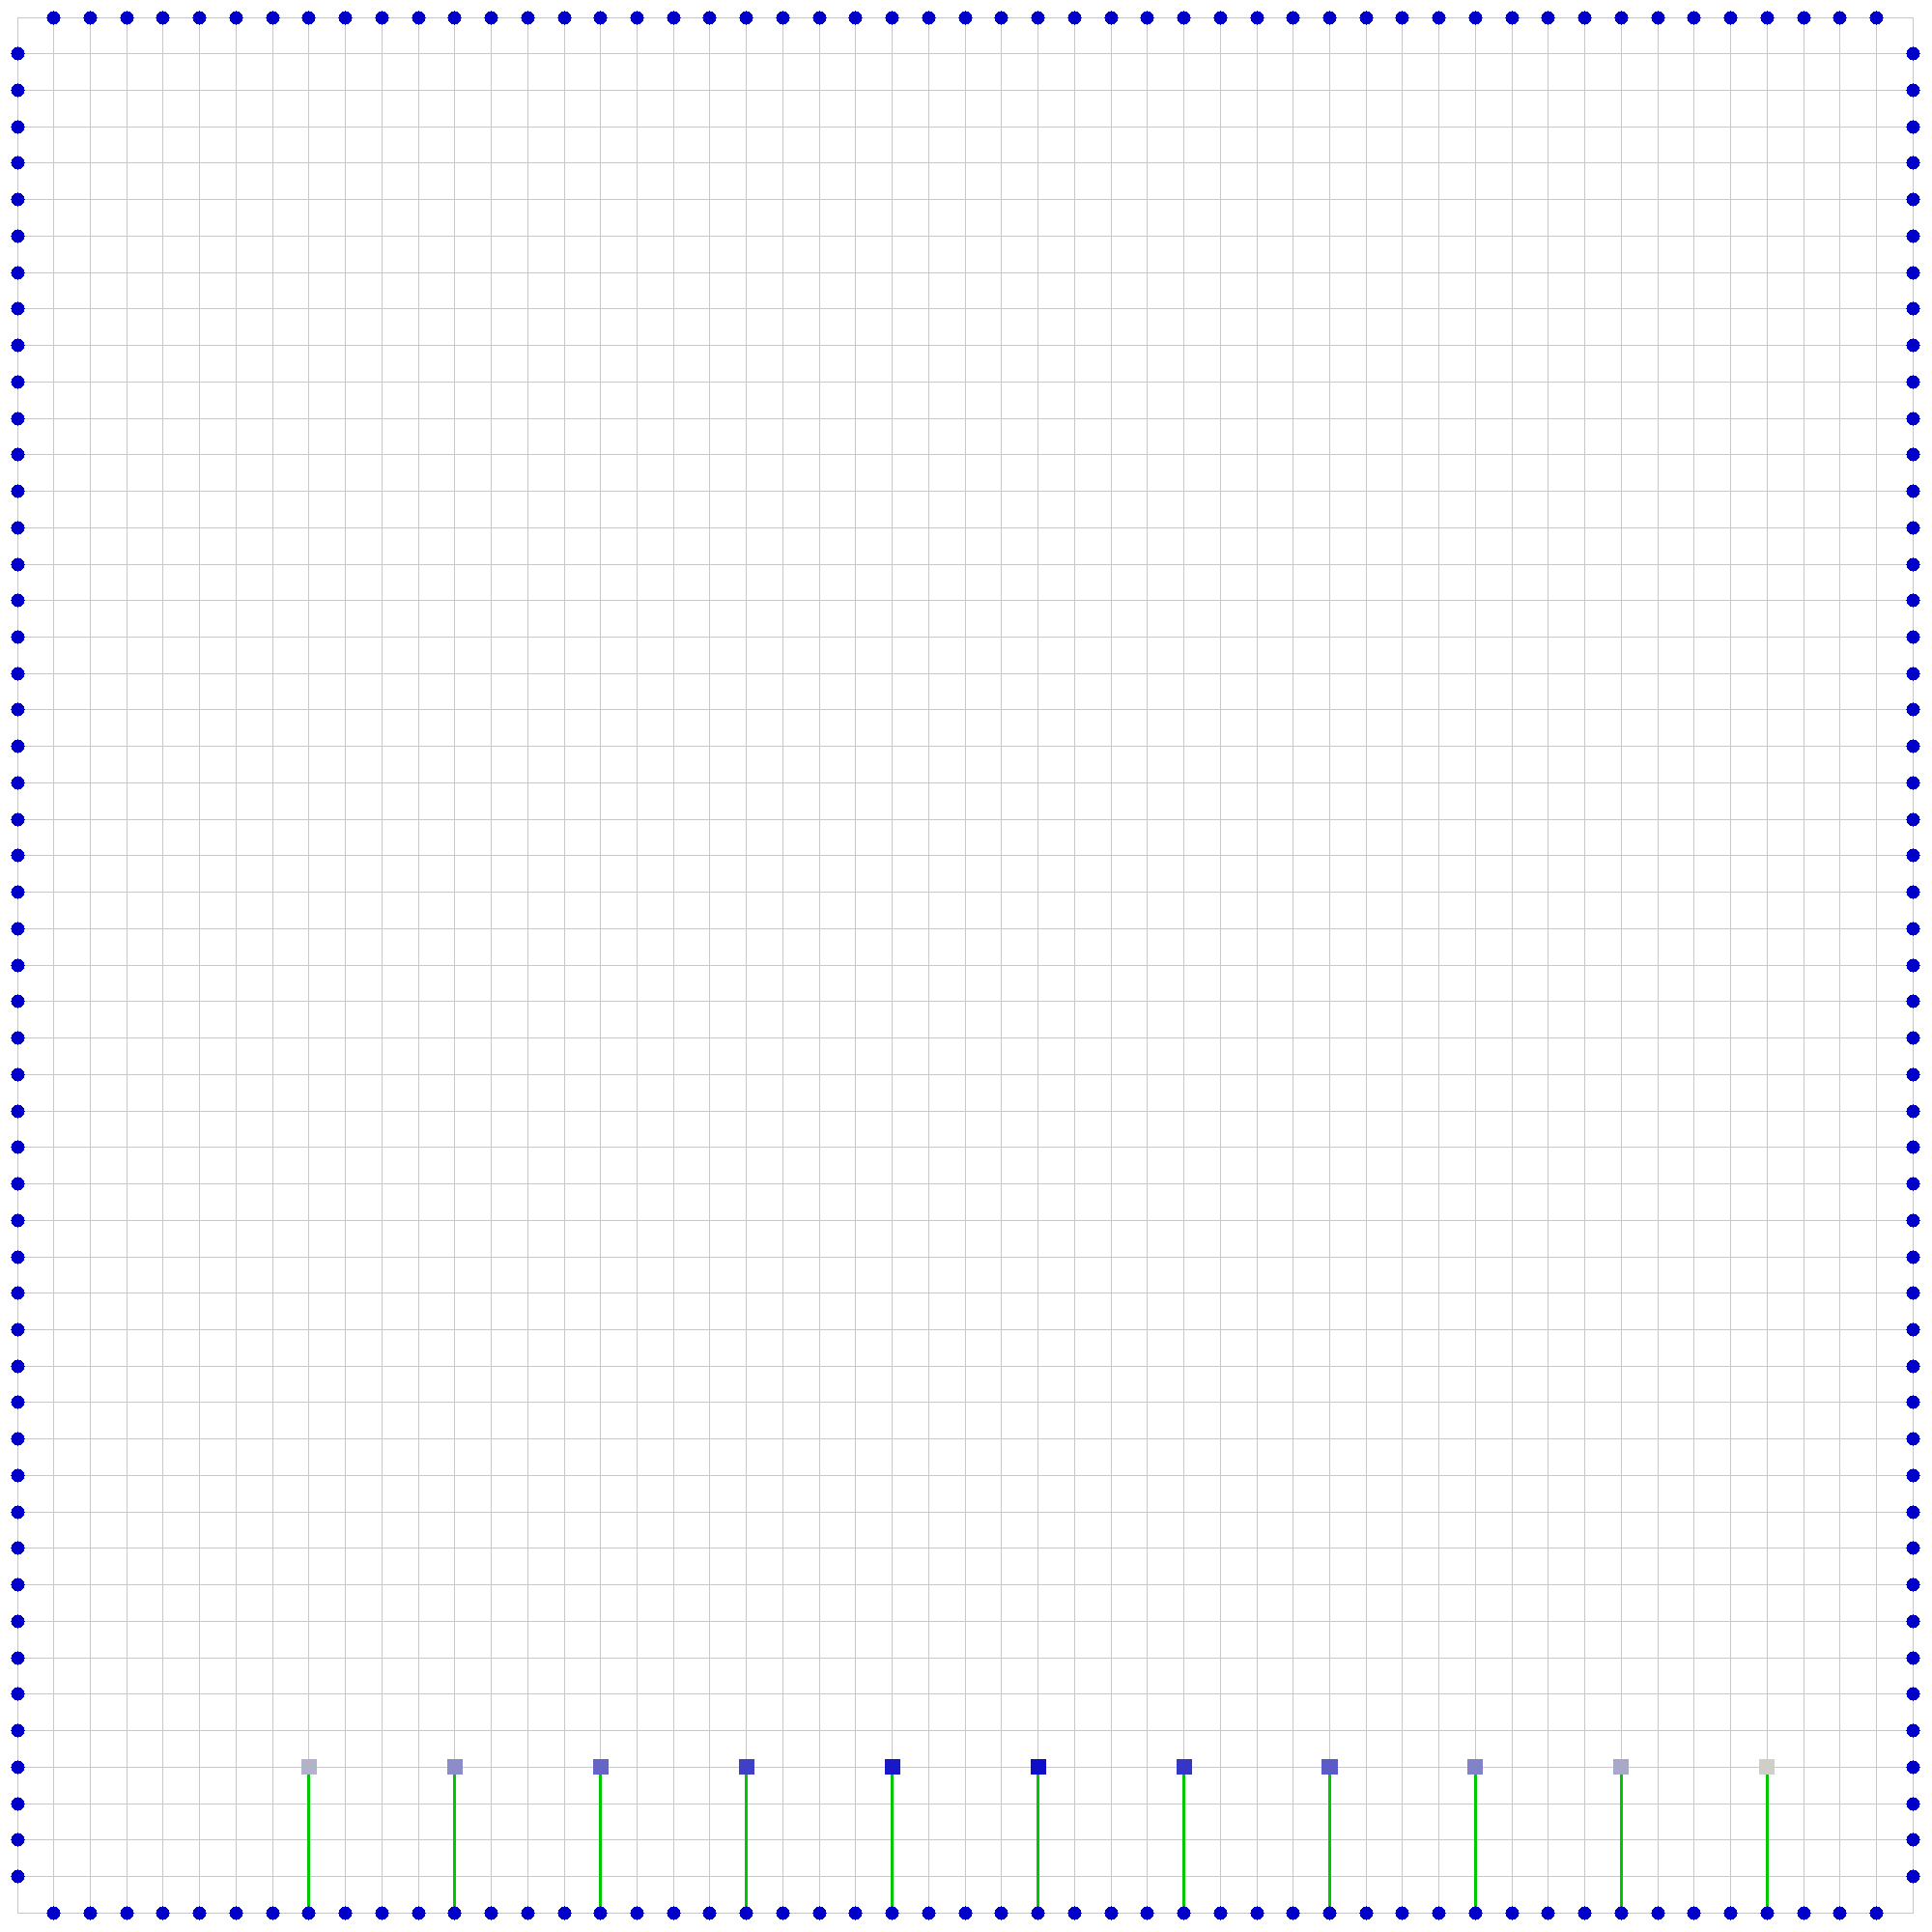
\includegraphics[width=2in]{12_1.png}
	\end{figure}
	\item 从最中间的部分,将三角形顶上的节点尽量连接出去。比如:
	\begin{figure}[H]
		\centering
		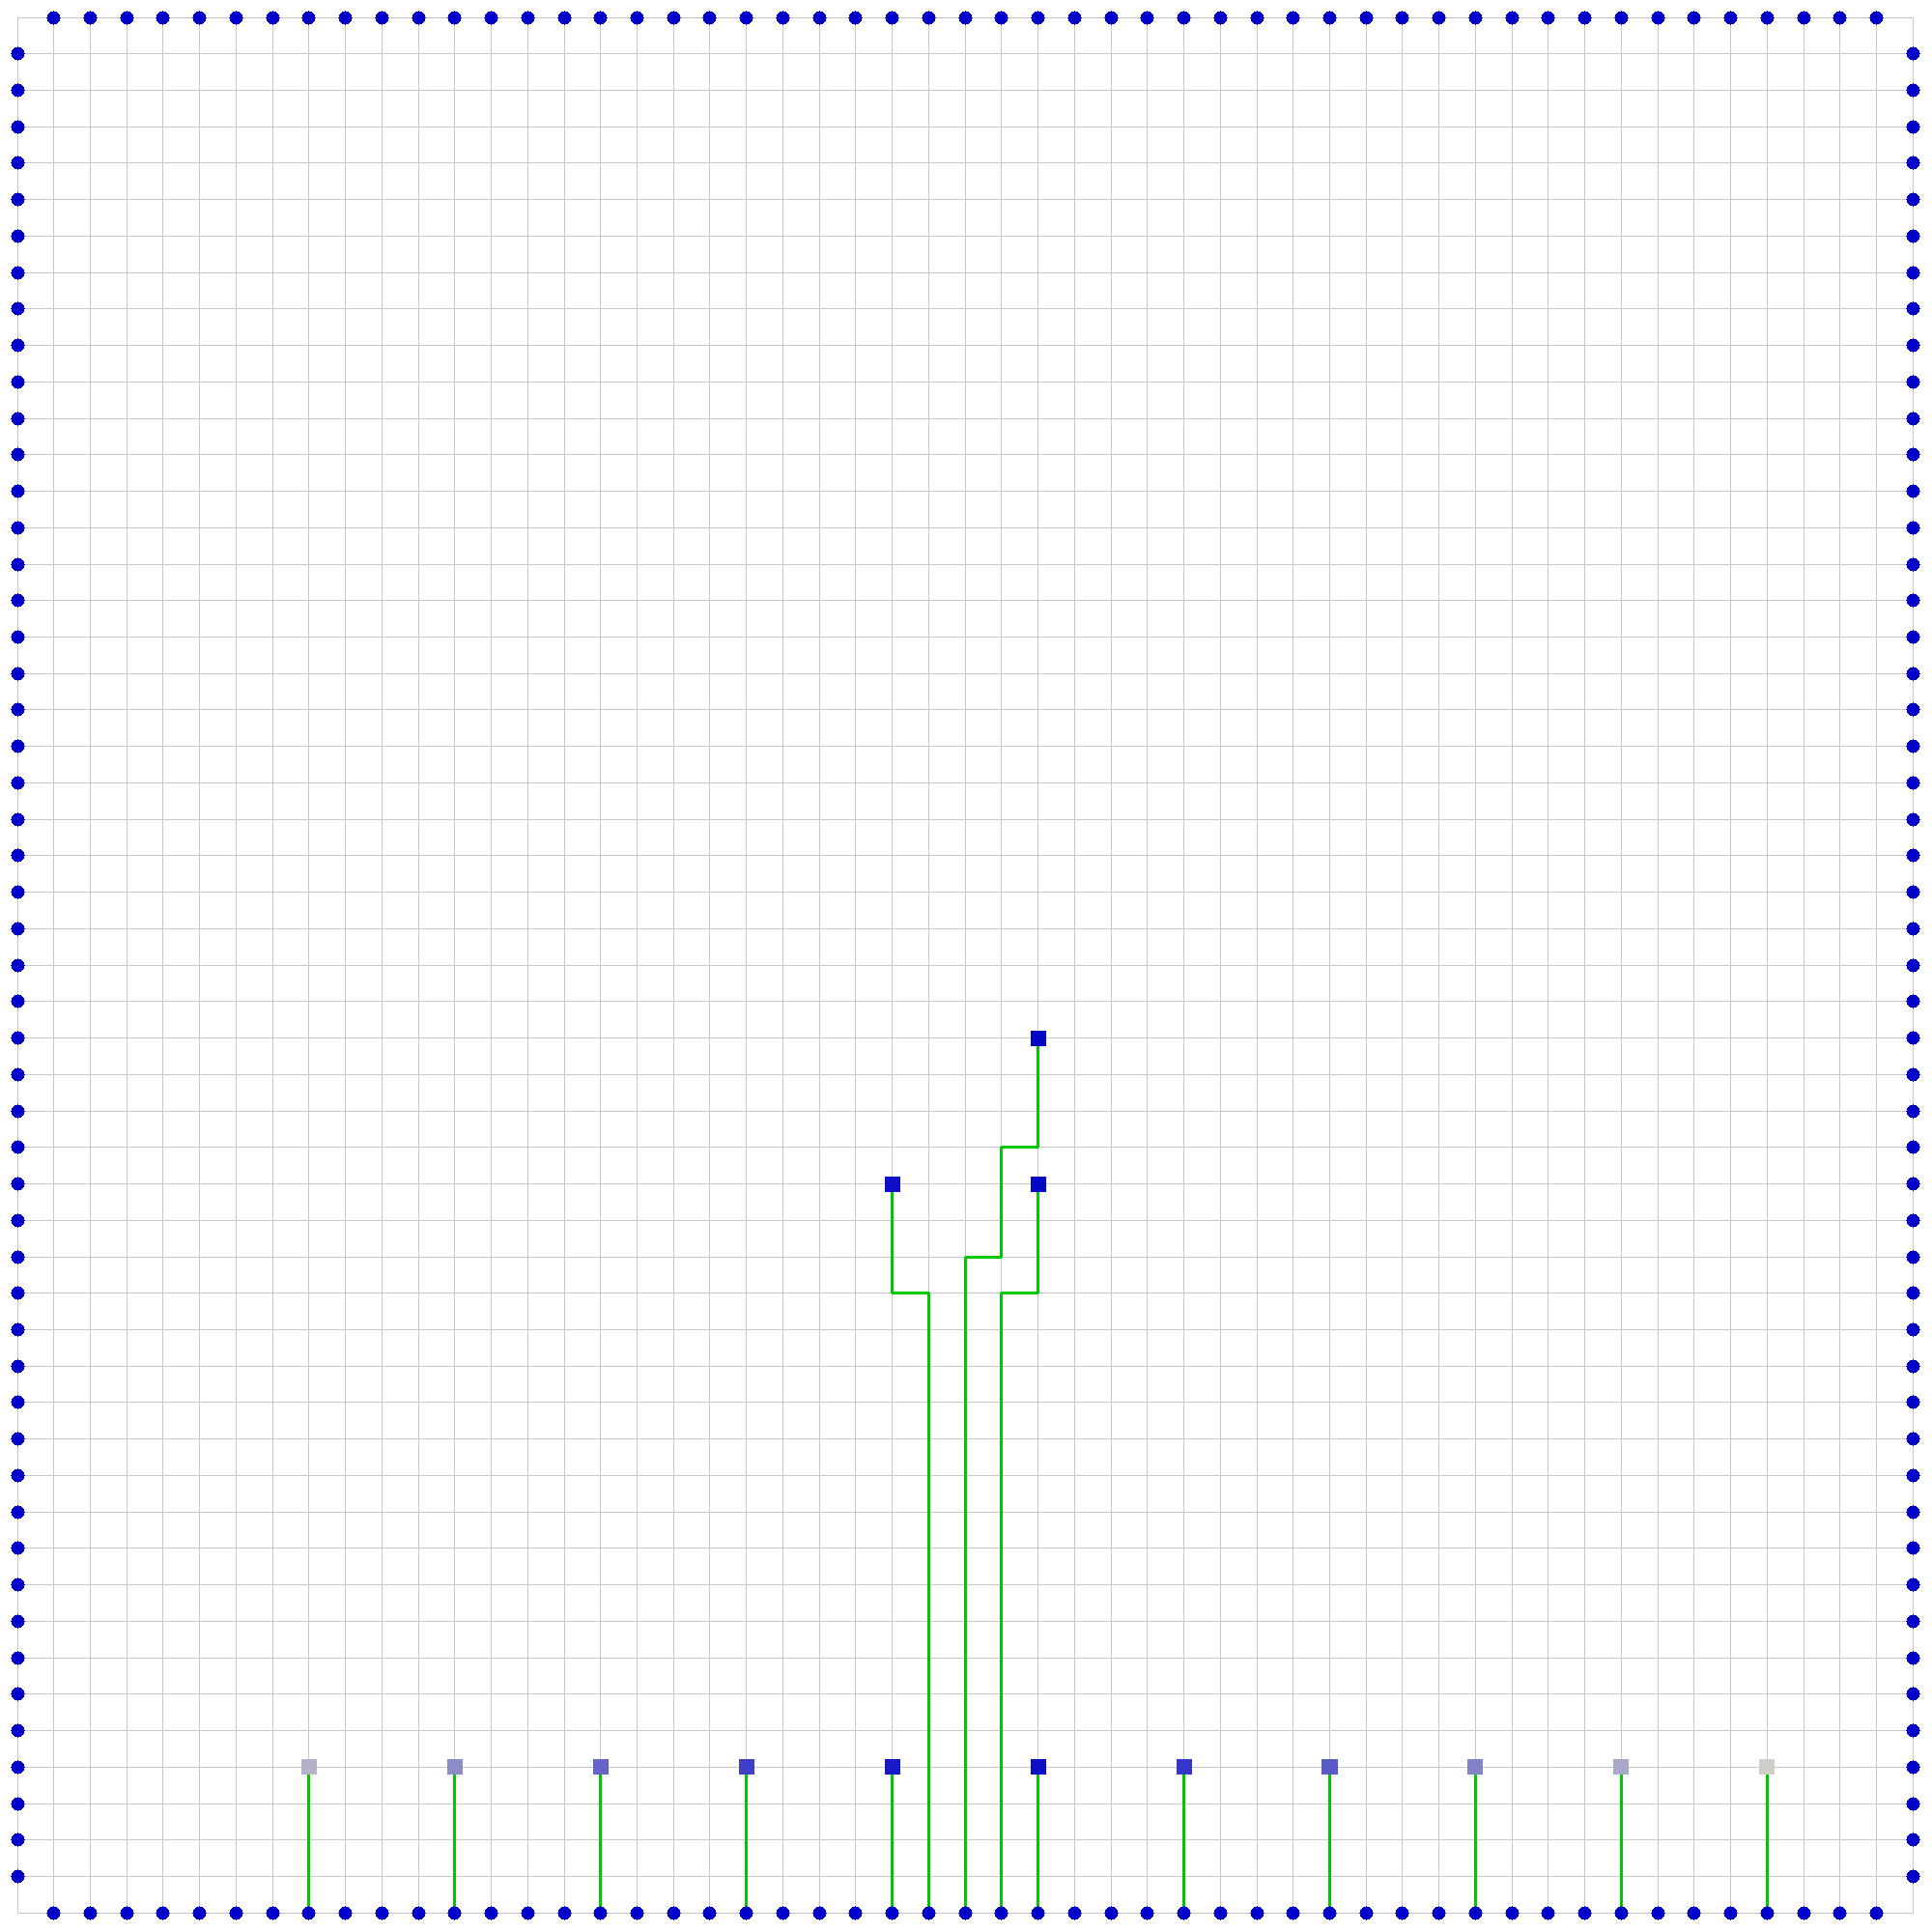
\includegraphics[width=2in]{12_2.png}
%		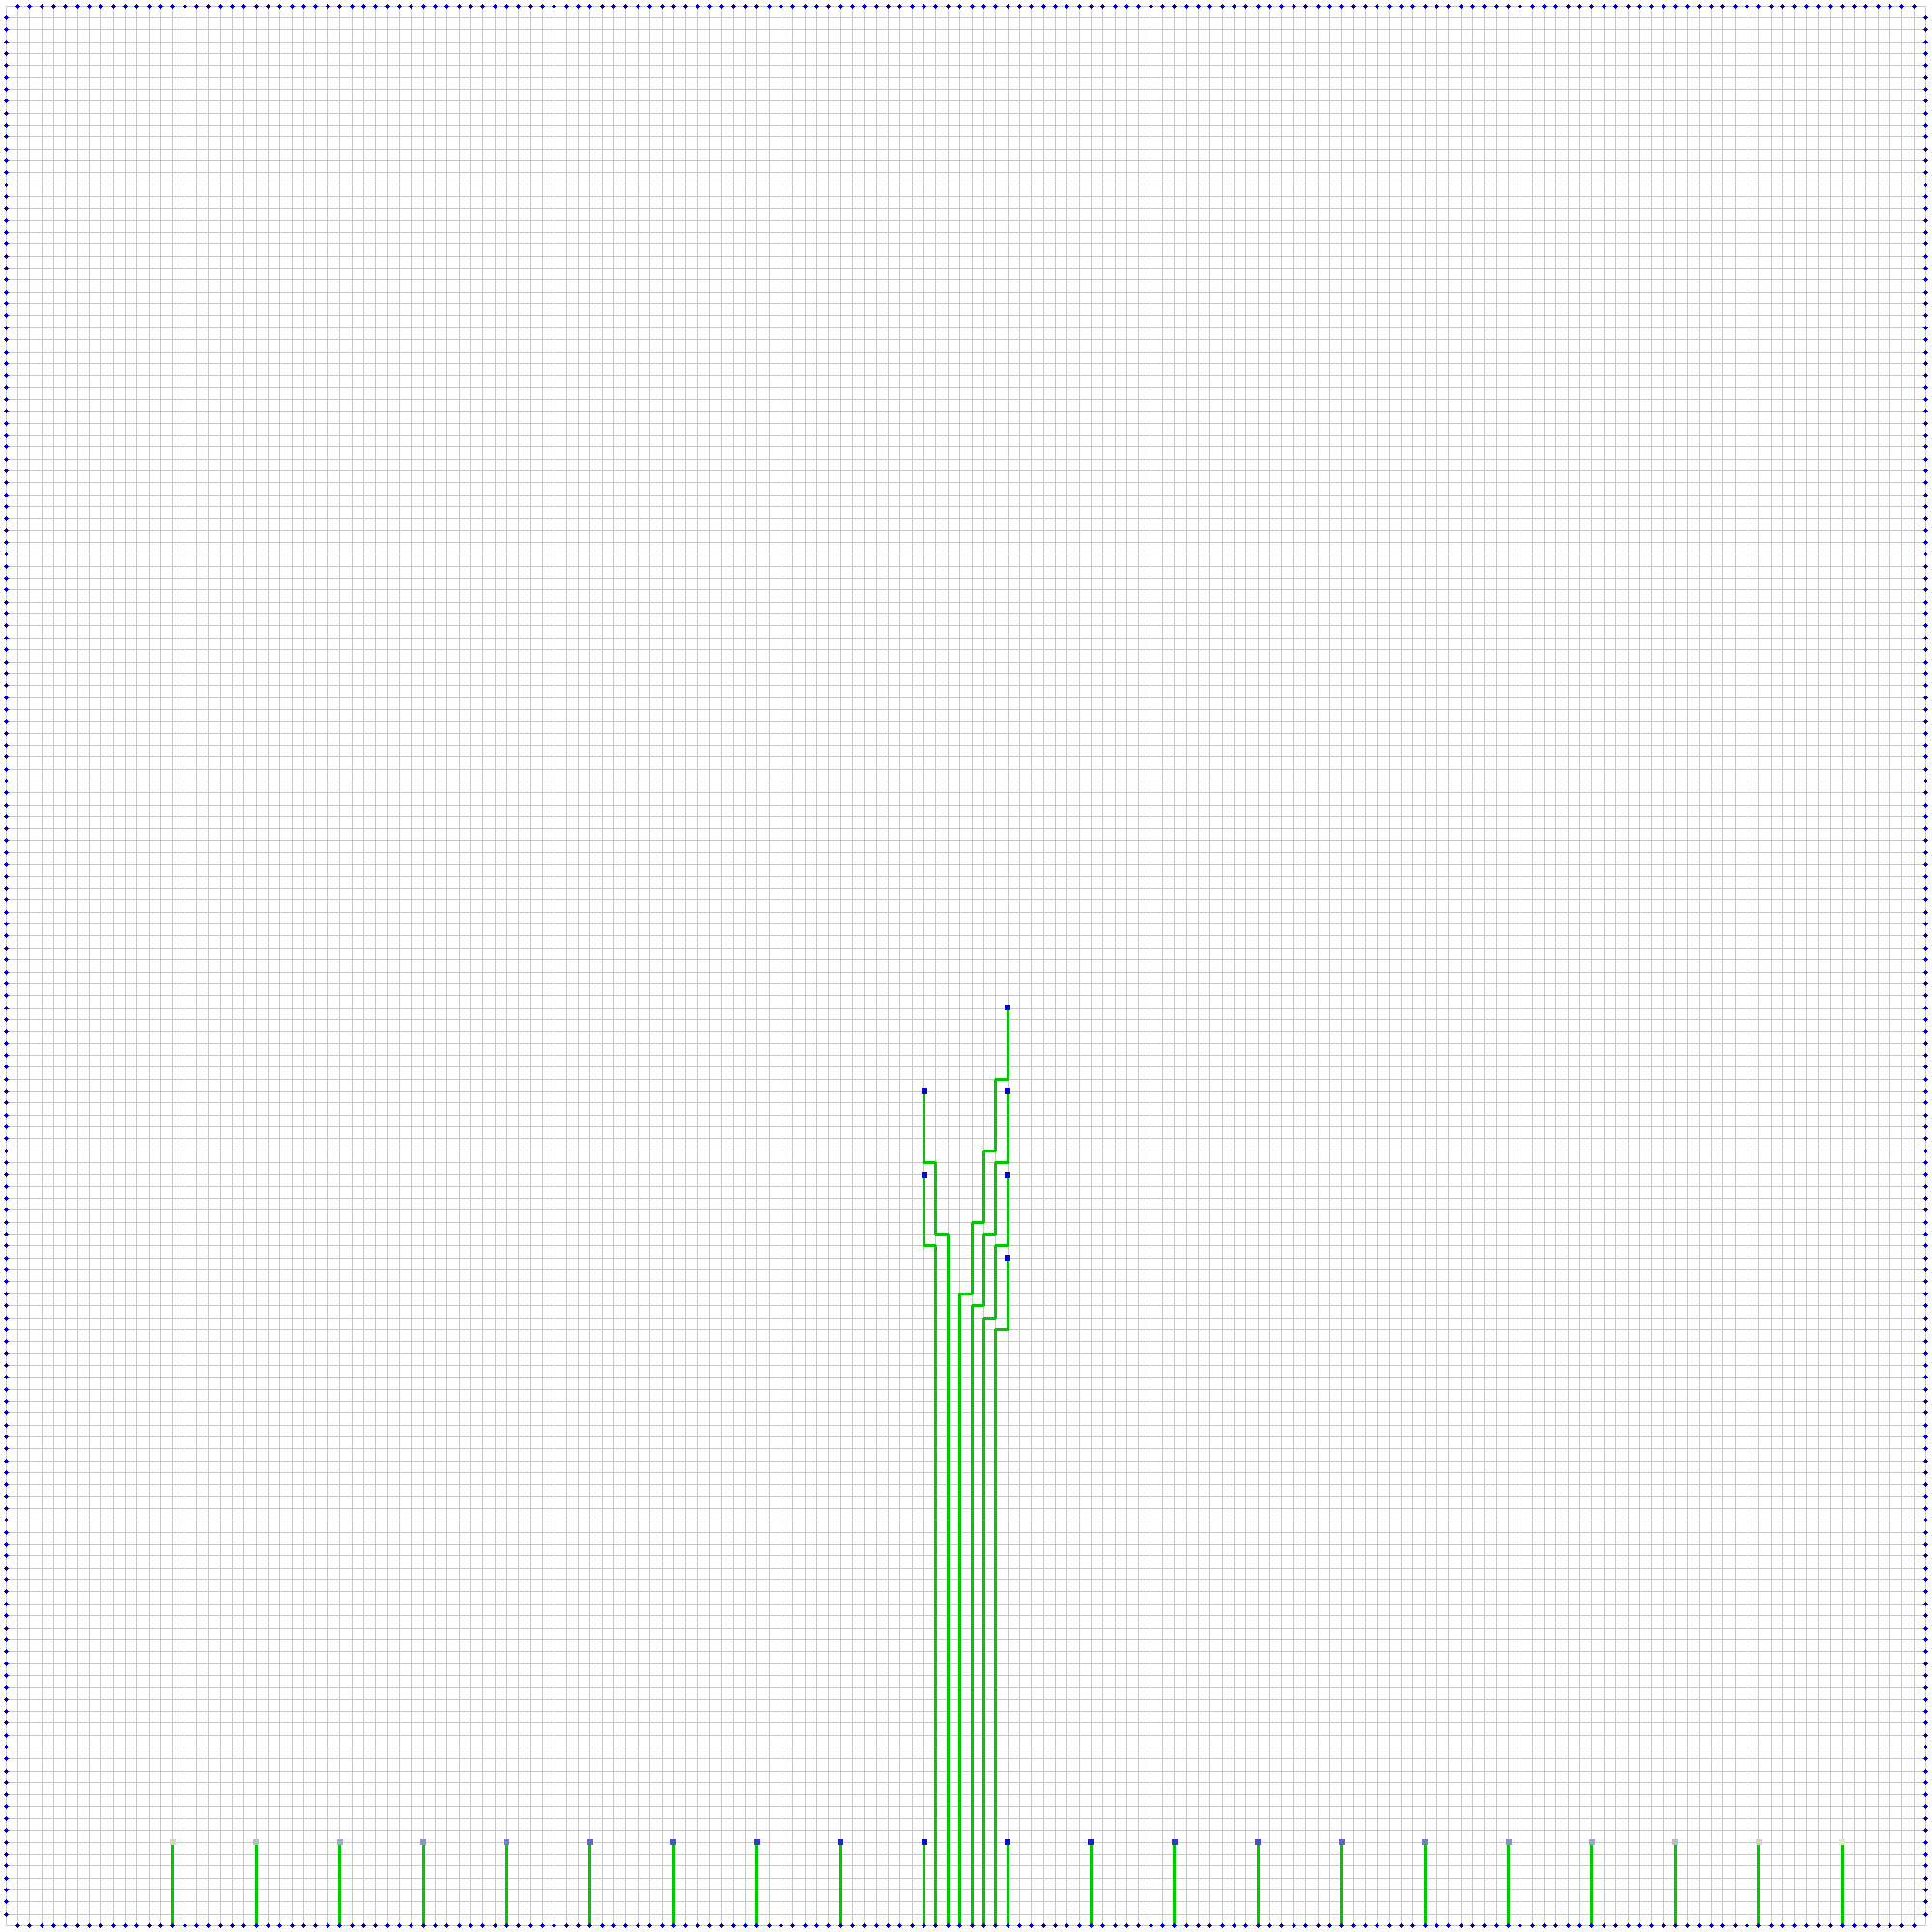
\includegraphics[width=2in]{22_2.png}
	\end{figure}
	\item 从中间向两边拓展。以左侧$\frac{1}{8}$的三角形为例,如果最右端还未被连接出去的点$A$可以执行连接操作,并且不会与其他尚未连接的点的连接发生冲突(即不存在某个点$B$,在$A$连接后,不存在任何一条路径,使得它能够被连接出去),那么就将$A$连接,并且出口尽量靠右。一个中间过程图如下图左图:
	\begin{figure}[H]
		\centering
		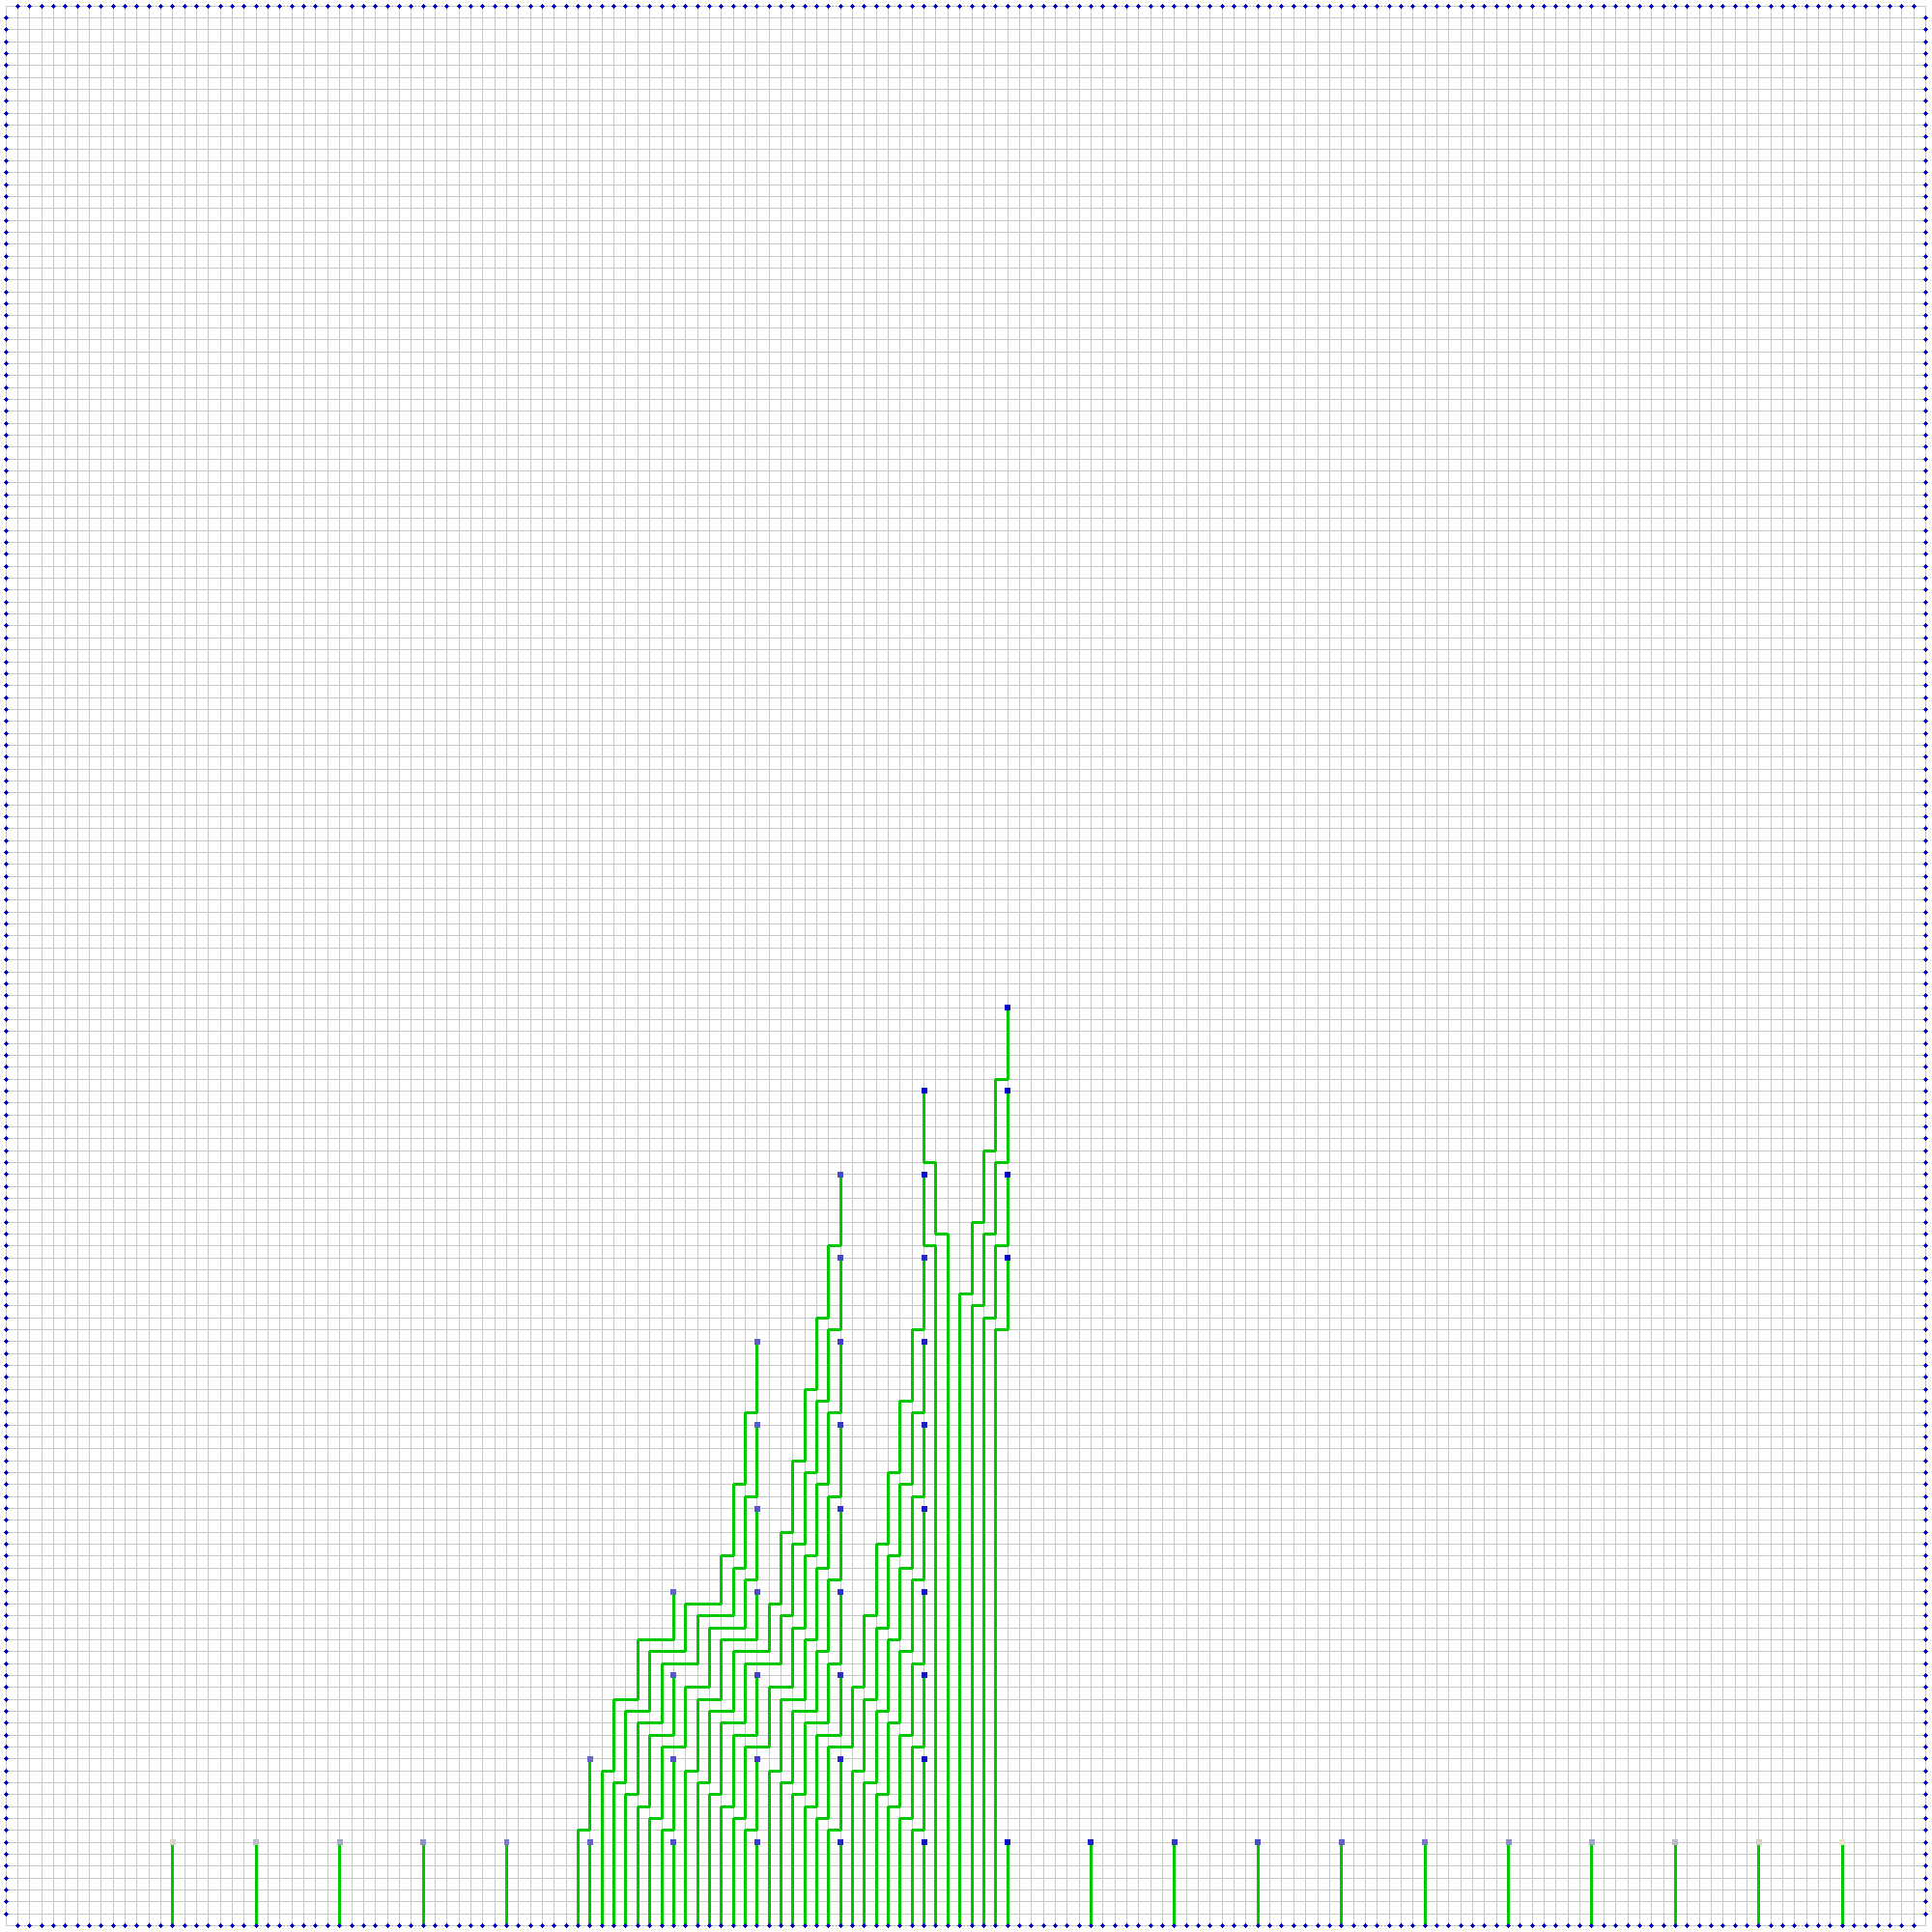
\includegraphics[width=2in]{22_3.png}
		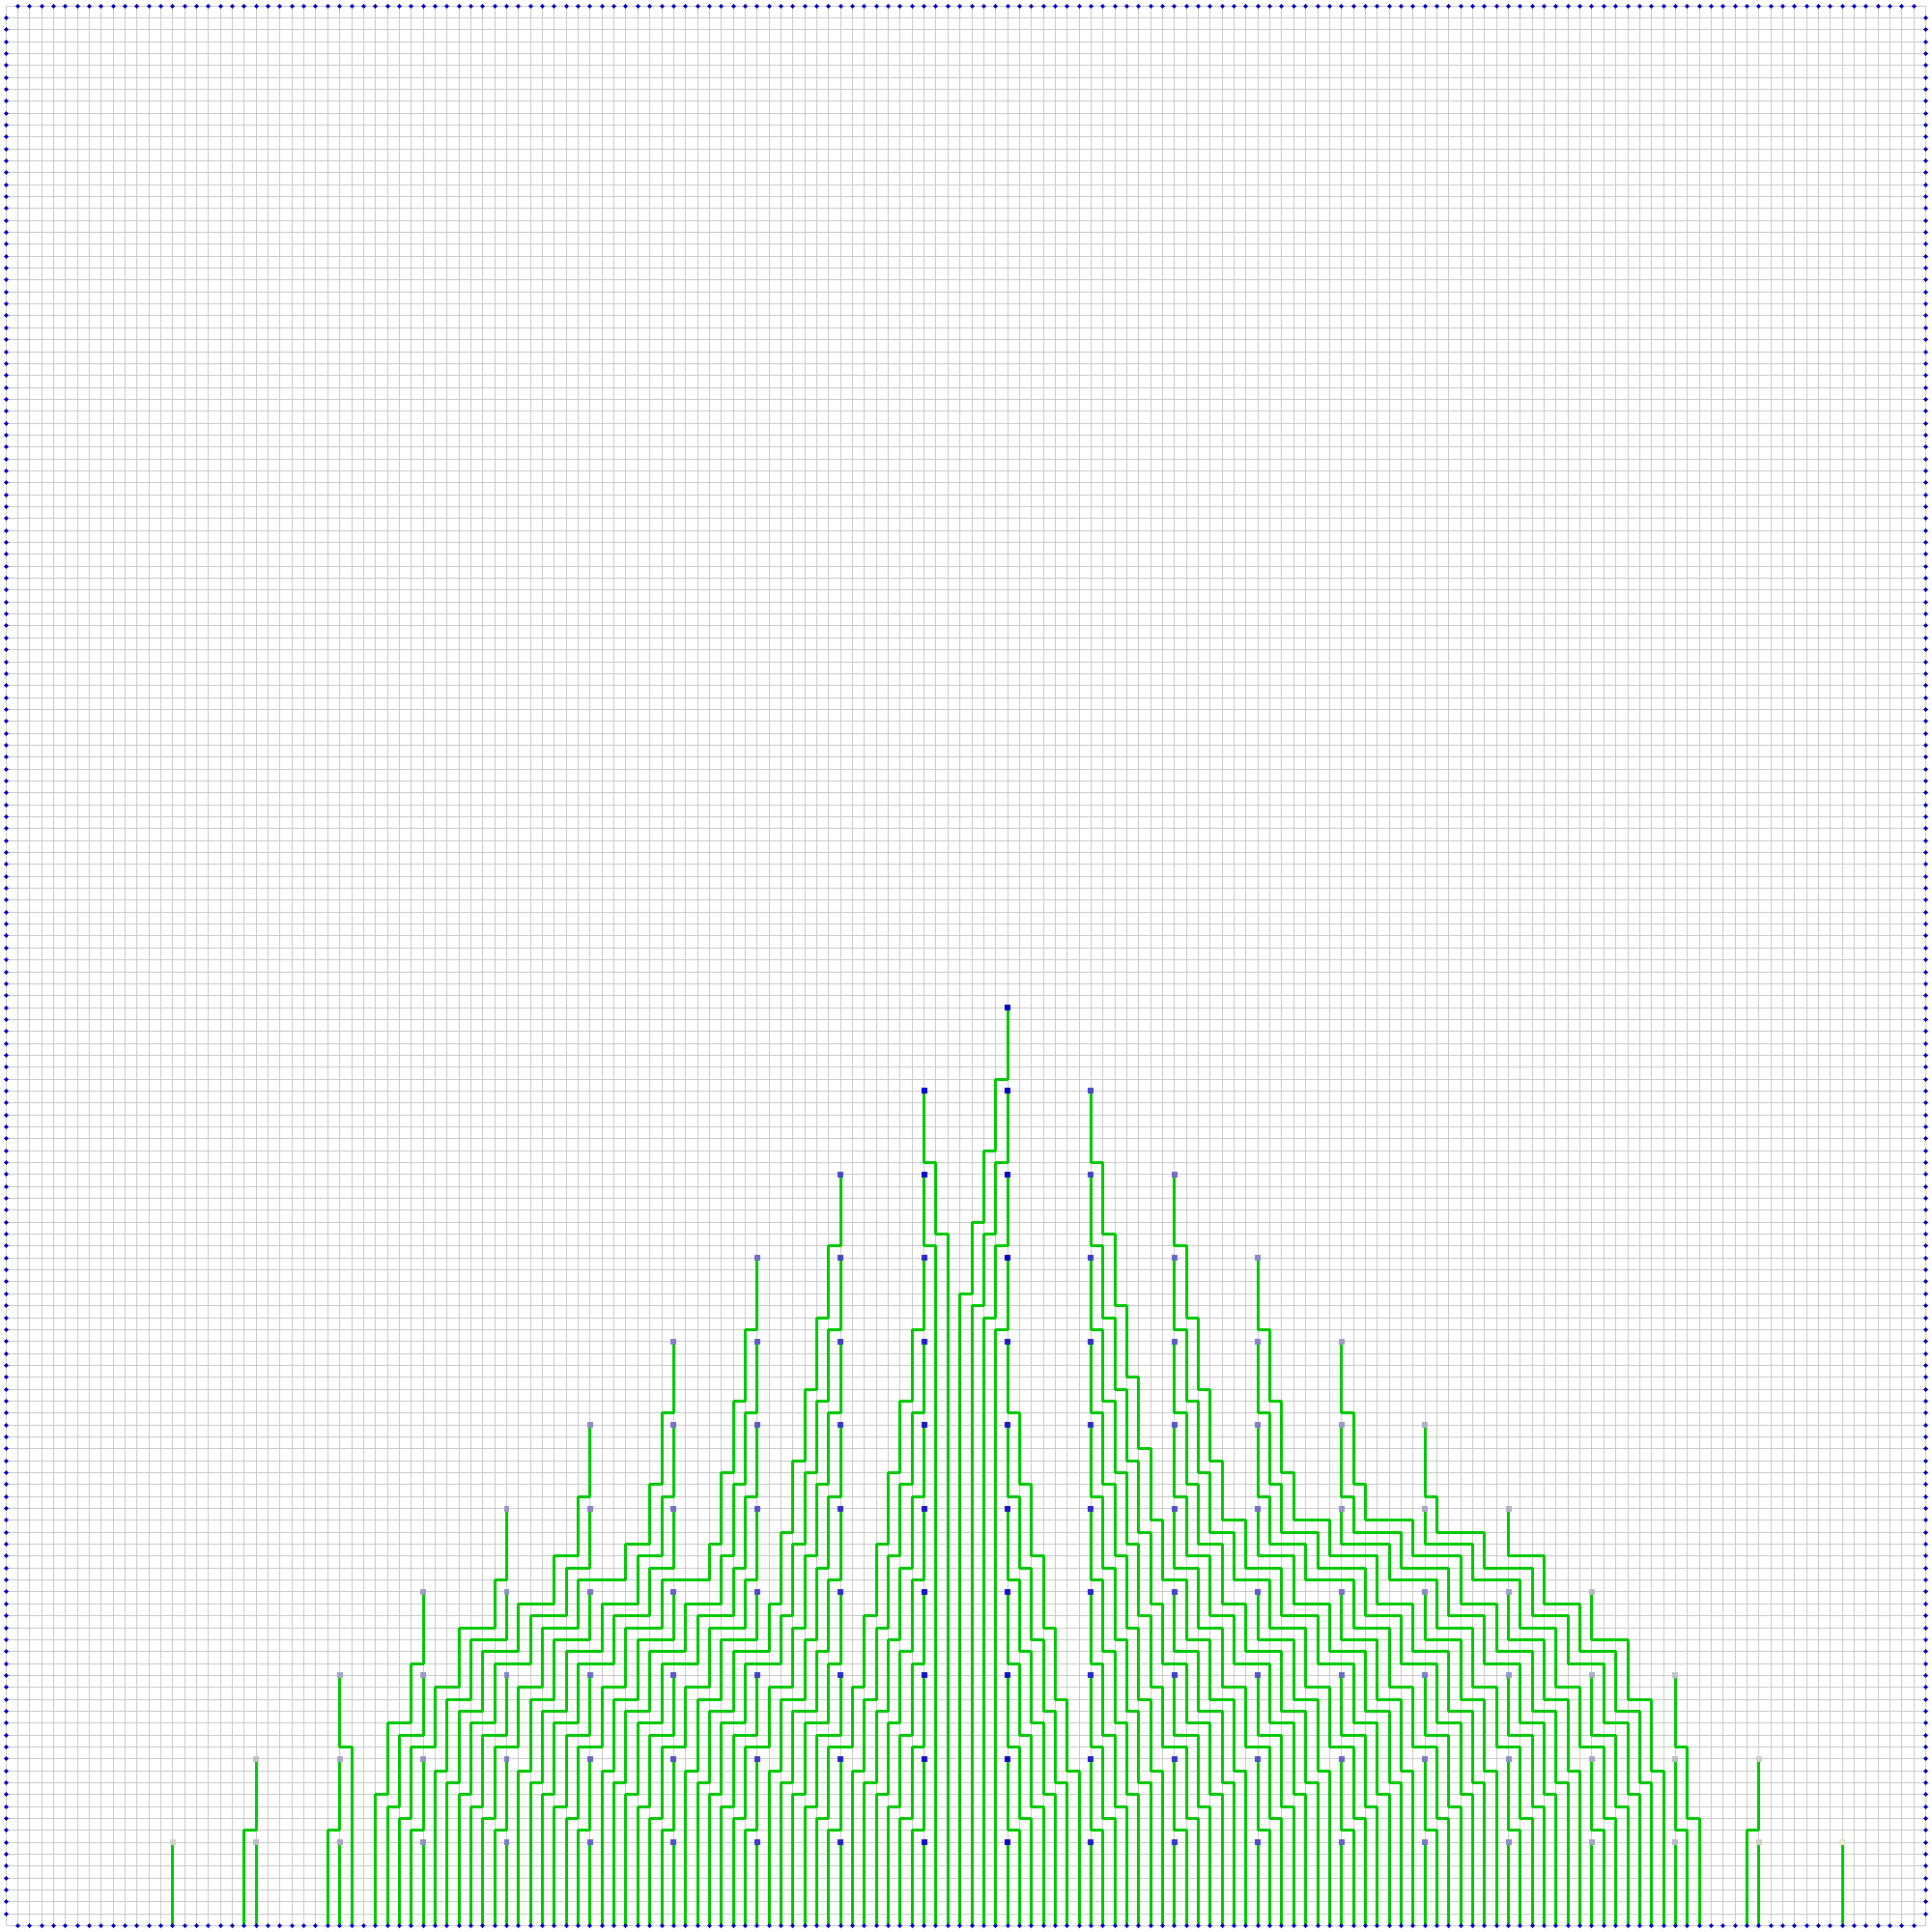
\includegraphics[width=2in]{22_4.png}
	\end{figure}	
	\item 处理两边角未被连接的节点。随便连一连就好了。最终这个$\frac{1}{4}$的三角形会变成上图右图那样。
	\item 最后将这四部的结果合并即可。
\end{enumerate}

在实现过程中,考虑到$80\times 80$的数据,网格图有$1945\times 1945$的大小,因此寻找路径的算法成为了效率实现的瓶颈。作者使用了$A^*$算法替代传统的BFS算法,估价函数设计成尽量贴着已存在的路径进行寻路,从而实现了效率正比于路径长度的高效算法。

经检验,该算法在$1\sim 80$的数据中只有两个数据需要一些微调,其他数据均快速出解,具体的效果详见下一章节。
